

\title{BSP Simulation}
\author{
        Quincy Wofford, Keira Haskins \\
}
\date{\today}

\documentclass[12pt]{article}
\usepackage{graphicx}

\begin{document}
\maketitle

\begin{abstract}
Reproducing work by Oscar Mondragon. We need to talk about a paper later. It's too early now!
\end{abstract}

\section*{Introduction}
This experiment is popperized
\section*{Method}
Singularity builds remotely, downloads, runs on local machine. Works on my local computer and Wheeler.
\section*{Results}
This section is broken down into Experiment results, where we look at data generated by the BSP simulator, and Pipeline results, where we inspect the experiment workflow diagram popper generated for us.
\subsection*{Experiment Results}
The results of the experiment itself may be viewed according to your needs. In this case, results are viewed in this \LaTeX document. The only thing about this document that changes after running the popper pipeline is the histogram seen below. It's possible to imagine scenarios where numeric results and many figures are stored in a file, then inserted into the paper. Some care when writing the paper must be taken to include the falsifiability goals. Clearly stating the implication, experiment result, with case statements to break down whether the newly generated paper does or does not violate evaluation thresholds.

\begin{center}
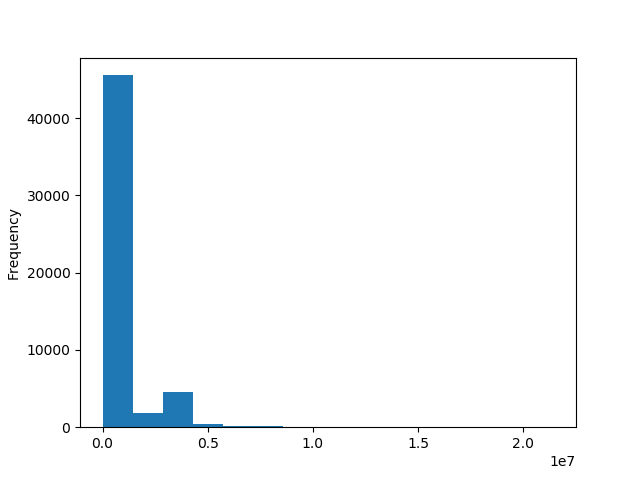
\includegraphics[scale=0.5]{../all_sample_hist.png} 
\end{center}

\subsection*{Pipeline Results}
The Popper pipeline generates results from its execution which may be found in your experiment folder under the popper/ directory. This is where you will find my setup and teardown notes, for instance. The popper pipeline will export error files and output files, so you'll want to check both to determine if your run was successful, or where your run failed.

\paragraph{}
Perhaps the most useful tool in creating my own pipeline was the experiment flowchart which popper automatically generates. This allows me to visualize the stages of the pipeline and their component parts.
\begin{center}
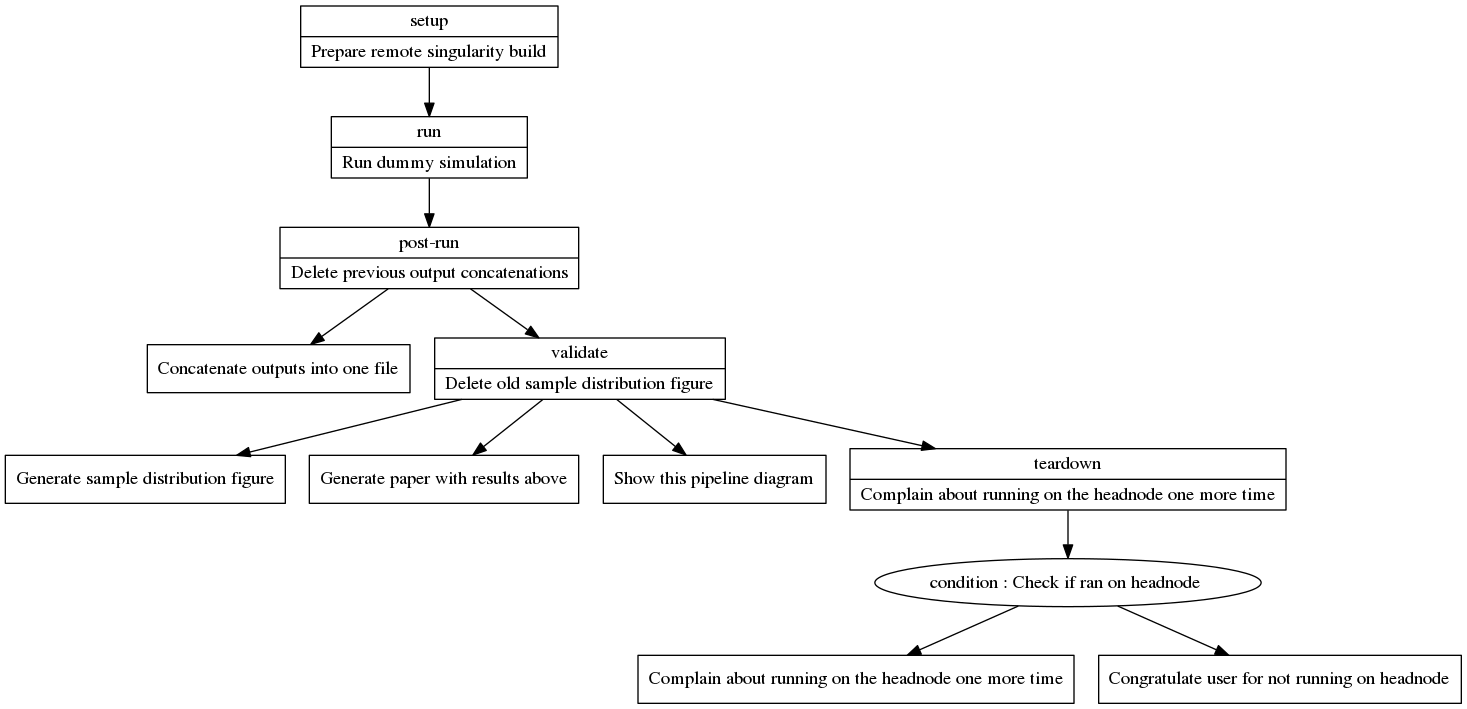
\includegraphics[scale=0.2]{../../wf.png}
\end{center}

\section*{Conclusion}
This experiment is Popperized. It takes some time to do, but it is a one-time time investment on the order of hours which will formalize our approach to reproducibility and enable us to gracefully deploy on many infrastructures.


\end{document}

